\documentclass[a4paper,12pt,twoside]{hmcpset}
\usepackage[utf8]{inputenc}
\usepackage[english]{babel}
\usepackage{fancyhdr}
\usepackage[margin=.8in]{geometry}
\usepackage{graphicx}
\usepackage{amsmath}
\usepackage{mathtools}
\usepackage[mathscr]{euscript}
\usepackage{lmodern} % math, rm, ss, tt
\usepackage[T1]{fontenc}
\usepackage{relsize}
\usepackage{mathtools}
\usepackage{tikz} 
\usepackage{tikz}\usetikzlibrary{arrows,patterns,calc,decorations.markings}
\usepackage{xintexpr}

%\newcommand*{\ms}[1]{\ensuremath{\mathscr{#1}}}
\renewcommand{\labelenumi}{{\bf (\alph{enumi})}}

\pagestyle{fancy}
\fancyhf{}
\rhead{Spring 2019}
\lhead{\vspace{5mm} Math 147 Topology}
\rfoot{Page \thepage}
\chead{Section 13}
 
\renewcommand{\headrulewidth}{2pt}
\renewcommand{\footrulewidth}{1pt}

\graphicspath{ {./figures_theorems/} } 

% info for header block in upper right hand corner
\begin{document}
\section*{Chapter 13\\ Fundamental Group: Capturing Holes}

\noindent

\begin{problem}[Theorem 13.2] 
    Given topological spaces $X$ and $Y$ with $S \subset X$, 
    homotopy relative to $S$ is an equivalence relation on the set of
    all the functions from $X$ to $Y$. In particular, if $S =
    \emptyset$, homotopy is an equvialence relation on the set of all
    continuous functions from $X$ to $Y$.
\end{problem}

\begin{proof}
    Let $f$ and $g$ be continuous functions from $X$ to $Y$. 
    Let us denote $f \simeq_S g$ to mean that $f$ and $g$ are homotopic
    relative to $S \subset X$.
    \begin{itemize}
        \item \textbf{Reflexive:} 
        Observe that this relation is reflexive. If $H(x, t) = f(x)$
        for all $t \in [0, 1]$, then it is trivial that $H$ forms a
        homotopy relative to $S$ between $f$ and itself.

        \item \textbf{Symmetric:} If $f \simeq_S g$, then there is a
        continuous function $H: X \times [0, 1] \to Y$ such that
        \begin{gather*}
            H(x, 0) = f(x) \qquad \text{ for all } x \in X\\
            H(x, 1) = g(x) \qquad \text{ for all } x \in X\\
            H(x, t) = f(x) = g(x) \qquad \text{ for all } x \in S, t \in [0, 1]
        \end{gather*}
        then consider $H(x, 1 -t)$ and observe that
        \begin{gather*}
            H(x, 1) = f(x) \qquad \text{ for all } x \in X\\
            H(x, 0) = g(x) \qquad \text{ for all } x \in X\\
            H(x, 1 - t) = f(x) = g(x) \qquad \text{ for all } x \in S, t \in [0, 1]
        \end{gather*}
        is a homotopy that deforms $g$ into $f$. Thus $g \simeq_S f$, so
        the relation is symmetric.

        \item \textbf{Transitive:} Now suppose $f \simeq_S g$ and $g \simeq_S h$.
        Then there exist continuous functions $H: X \times [0, 1] \to
        Y$ and $G : X \times [0, 1] \to Y$ such that 
        \begin{gather*}
            H(x, 0) = f(x) \qquad \text{ for all } x \in X\\
            H(x, 1) = g(x) \qquad \text{ for all } x \in X\\
            H(x, t) = f(x) = g(x) \qquad \text{ for all } x \in S, t \in [0, 1]
        \end{gather*}
        and 
        \begin{gather*}
            G(x, 0) = g(x) \qquad \text{ for all } x \in X\\
            G(x, 1) = h(x) \qquad \text{ for all } x \in X\\
            G(x, t) = g(x) = h(x) \qquad \text{ for all } x \in S, t \in [0, 1].
        \end{gather*}
        Now observe that we can construct the function
        \[
           F =
           \begin{cases}
               H(x, 2t) & 0 \le t \le \frac{1}{2}\\
               G(x, 2t - 1) & \frac{1}{2} < t \le 1
           \end{cases} 
        \]
        which will be a homotopy relative to $S$ from $f$ to $h$. Note
        that continuity here is guaranteed by application of the
        pasting lemma, since $H$ and $G$ are continuous on the same intervals. 
        In total, we then have that $f \simeq_S g$ and $g \simeq_S h$
        imply $f \simeq_S h$, as desired.
    \end{itemize}
\end{proof}

\begin{problem}[Theorem 13.3]
    If $\alpha, \alpha', \beta$ and $\beta'$ are paths in a space $X$
    such that $\alpha \sim \alpha'$, $\beta \sim \beta'$ and
    $\alpha(0) = \beta(1)$, then $\alpha \cdot \beta \sim \alpha'
    \cdot \beta'$.  
\end{problem}

\begin{proof}
    Since $\alpha \sim \alpha'$ and $\beta \sim \beta'$, there exists
    homotopies $A$ and $B$ which connect $\alpha$ to $\alpha'$ and
    $\beta$ to $\beta'$. Consider the continuous function 
    \[
        H(x, t) =
        \begin{cases}
            A(2x, t) \quad 0 \le x \le \frac{1}{2}\\
            B(2x - 1, t) \quad \frac{1}{2} < x \le 1
        \end{cases}  
    \]
    which is a homotopy from $\alpha \cdot \beta$ to $\alpha' \cdot
    \beta'$ since $H(x, 0) = \alpha(x)\cdot \beta(x)$, $H(x, 1) =
    \alpha'(x)\cdot \beta'(x)$, $H(0, t) =\alpha(0) = \alpha'(0)$ 
    and $H(1, t) = \beta(0) = \beta'(0)$.
    
    
\end{proof}

\begin{problem}[Theorem 13.4]
    Given paths $\alpha, \beta$ and $\gamma$ where the following
    products are defined, then  
    $(\alpha \cdot \beta) \cdot \gamma \sim (\beta \cdot
    \gamma) \cdot \alpha$ and $([\alpha] \cdot [\beta])\cdot [\gamma]
    = [\alpha]\cdot([\beta] \cdot [\gamma])$
\end{problem}  

\begin{proof}
    Consider the homotopy given by 
    \[
        H(x, t) = 
        \begin{cases}
            \alpha\left( \dfrac{4x}{2 - t} \right) & 0 \le x \le \dfrac{2 - t}{4}\\
            \beta(4x + t -2) & \dfrac{2 - t}{4} \le x \le \dfrac{3 - t}{4} \\
            \\
            \gamma\left( \dfrac{4x - 3 + t}{1 + t} \right) & \dfrac{3 - t}{4} \le x \le 1.
        \end{cases}        
    \]
    Observe that 
    \[
        H(x, 0) = 
        \begin{cases}
            \alpha(2x) & 0 \le x \le \frac{1}{2}\\
            \beta(4x - 2) & \frac{1}{2} \le x \le \frac{3}{4}\\
            \gamma(4x - 3) & \frac{3}{4} \le x \le 1
        \end{cases}
        = \alpha \cdot (\beta \cdot \gamma)
    \]
    and 
    \[
        H(x, 1) = 
        \begin{cases}
            \alpha(2x) & 0 \le x \le \frac{1}{4}\\
            \beta(4x - 2) & \frac{1}{4} \le x \le \frac{1}{2}\\
            \gamma(4x - 3) & \frac{1}{2} \le x \le 1
        \end{cases}
        = (\alpha \cdot \beta) \cdot \gamma.
    \]
    Thus we see that $H$ is continuous by the pasting lemma, $H(x, 0) = \alpha \cdot(\beta
    \cdot \gamma)$ and $H(x, 1) = (\alpha \cdot \beta) \cdot \gamma$.
    In addition, we see that $H(0, t) =\alpha \cdot (\beta \cdot
    \gamma)(0) = (\alpha \cdot \beta) \cdot \gamma(0)$ 
    and 
    $H(1, t) = (\alpha \cdot \beta) \cdot \gamma(1) = \alpha \cdot (\beta \cdot
    \gamma)(1)$. Thus we have that 
    $\alpha \cdot (\beta \cdot \gamma) \sim (\alpha \cdot \beta) \cdot
    \gamma$, which implies that 
    \[
        [\alpha \cdot (\beta \cdot \gamma)] = [(\alpha \cdot \beta) \cdot \gamma]
    \]
    as desired.

\end{proof}

\begin{problem}[Theorem 13.5]
    Let $\alpha$ be a path with $\alpha(0) = x_0$. Then $\alpha \cdot
    \alpha^{-1} \sim e_{x_0}$, where $e_{x_0}$ is the constant path at
    $x_0$. 
\end{problem}

\begin{proof}
    Consider the homotopy
    \[
        H(x, t) = 
        \begin{cases}
            \alpha(2x)  & 0 \le x \le \frac{1 - t}{2}\\
            \alpha^{-1}(2x - 1) & \frac{1-t}{2} \le x \le 1-t\\
            e_{x_0} & 1-t \le x \le 1.
        \end{cases}
    \]
    which traverses $\alpha, \alpha^{-1}$, and then sits at $x_0$.
    Observe that 
    \[
        H(x, 0) = 
        \begin{cases}
            \alpha(2x) & 0 \le x \le \frac{1}{2}\\
            \alpha^{-1}(2x - 1) & \frac{1}{2} \le x \le 1.
        \end{cases} = \alpha \cdot \alpha^{-1}
    \]
    while 
    \[
        H(x, 1) = e_{x_0} \quad 0 \le x \le 1.
    \]
    In addition, we have that $\alpha \cdot \alpha^{-1}(x) =
    e_{x_0}(x)$ for $x = 0, 1$. Also, $H$ is continuous by the pasting
    lemma. Thus we have that 
    \[
        \alpha \cdot \alpha^{-1} \sim e_{x_0}
    \] 
    as desired. The proof is nearly identitical to show that $\alpha^{-1}
    \cdot \alpha \sim e_{x_0}$.

\end{proof}

\begin{problem}[Theorem 13.6]
    The fundamental group $\pi_1(X, x_0)$ is a group. The identity
    element is the class of homotopolically trivial loops based at $x_0$.
\end{problem}

\begin{proof}
    \begin{description}
        \item[Identity.] With a group operation $\cdot$, we see that there is an identity
        element $e_{x_0}$ such that $[\alpha] \cdot [\alpha^{-1}] =
        [\alpha^{-1}] \cdot [\alpha] = [e_{x_0}]$ 
        
        \item[Associativity.] We have associativity of products by Theorem 13.4. 
        
        \item[Inverse Elements.] Inverse elements exist by simply defining $\alpha^{-1}(t) = \alpha(1
        - t)$. This will still be loop about $x_0$, and hence will
        continue to be a member of $\pi_1(X, x_0)$.

        \item[Closure.] Finally, observe that the product is closed in the group, since
        any sequence of loops about $x_0$, their product
        \[
            [\alpha_{1}]\cdot[\alpha_{2}]\cdot \vspace{0.01mm} \dots \vspace{0.01mm} \cdot [\alpha_{n}] = [\alpha_1 \cdot \alpha_{2} \cdot  \vspace{0.01mm} \dots \vspace{0.01mm}  \cdot \alpha_{n}]
        \]
        will itself be a loop about
        $x_0$, and hence by definition., an element which is already in
        the set. Thus the fundamental group $\pi_1(X, x_0)$ is in fact
        a group.
    \end{description}    





\end{proof}

\begin{problem}[Theorem 13.7]
    If $X$ is path connected, then $\pi_1(X, p) \cong \pi_1(X, q)$
    where $p, q \in X$.
\end{problem}

\begin{proof}
    We'll do this by constructing a bijective homomorphism. Since $X$
    is path connected, there must exist a path $\gamma$ from $p$ to
    $q$. Let $\alpha$ and $\beta$ be loops centered at $p, q$
    respectively. Then observe that the function $ \psi :\pi_1(X, p) \to
    \pi_1(X, q)$ defined as
    \[
        \psi[\alpha] = \gamma^{-1}\alpha\gamma  
    \]
    is a homomorphism, since if $\alpha_1, \alpha_2 \in \pi_1(X, p)$,
    \[
        \psi[\alpha_1\alpha_2] = \gamma^{-1}\alpha_1\alpha_2\gamma
        = \gamma^{-1}\alpha_1\gamma \gamma^{-1}\alpha_2\gamma
        = \psi[\alpha_1]\psi[\alpha_2].
    \]
    We can similarly construct a homomorphism $\phi: \pi_1(X, q) \to
    \pi_1(X, p)$ as 
    \[
        \phi[\beta] = \gamma\beta\gamma^{-1}. 
    \]
    The proof is exactly the same as before: let $\beta_1, \beta_2 \in
    \pi_1(X, q)$. Then
    \[
        \phi[\beta_1\beta_2] = \gamma\beta_1\beta_2\gamma^{-1}
        = \gamma\beta_1\gamma^{-1} \gamma\beta_2\gamma^{-1}
        = \phi[\beta_1]\phi[\beta_2].
    \]
    Now observe that this homomorphism we constructed is in fact the
    inverse of $\psi$, since 
    \begin{gather*}
        \psi(\phi(\beta))= \gamma^{-1}\phi(\beta)\gamma = \gamma^{-1}\gamma\beta\gamma^{-1}\gamma = \beta\\
        \phi(\phi(\alpha)) = \gamma\phi(\alpha)\gamma^{-1} = \gamma\gamma^{-1}\alpha\gamma\gamma^{-1} = \alpha.
    \end{gather*}
    Therefore, $\psi$ is a bijective homomorphism, which proves that 
    $\pi_1(X, p) \cong \pi_1(X, q)$.
    
\end{proof}

\begin{problem}[Corollay 13.8]
    Suppose $X$ is a topological space and there is a path between the
    points $p$ and $q$ in $X$. Then $\pi_1(X, p)$ is isomorphic to 
    $\pi_1(X, q)$.
\end{problem}

\begin{proof}
Observe that this result is immediate since the proof of Theorem 13.7
relied on the fact that there exists a path between $p$ and $q$. Thus
the proof can be used exactly the same to show that path connectedness
between two points is sufficient to guarantee that $\pi_1(X, p) \simeq
\pi_1(X, q)$.


\end{proof}

\begin{exercise}[Exercise 13.9]
Let $\alpha$ be a loop into a topological
space $X$. Then $\alpha = \beta \circ \omega|_{[0,1]}$ where $
\omega$ is the standard wrapping map and $\beta$ is some continuous
function from $\mathbb{S}^1$ into $X$. This relationship gives a
correspondence between loops in $X$ and continuous maps from
$\mathbb{S}$ into $X$.
\end{exercise}

\begin{solution}
Consider the function $\omega^{-1} : \mathbb{S} \to [0, 1]$ where
$\omega(0) = \omega(1)$. As this is a continuous function, we then see
that $\alpha \circ \omega^{-1} : \mathbb{S} \to X$ is a continuous
function that maps out the curve $X$. Define this to be $\beta$. Then
observe that we can write this as 
\[
    \beta = \alpha \circ \omega^{-1} \implies \alpha = \beta \circ \omega  
\]
so that $\alpha$ can be written as a continuous from from $\mathbb{S}
\to X$ composed with a continuous function from $[0, 1] \to
\mathbb{S}$, as desired.
\end{solution}

\begin{problem}[Theorem 13.10]
    Let $X$ be a topological space and let $p$ be a point in $X$.
    Then a loop $\alpha = \beta \circ \omega|_{[0, 1]}$ (where
    $\omega$ is the standard wrapping map and $\beta$ is a continuous
    function from $\mathbb{S}^1$ into $X$) is homotopically trivial if
    and only if $\beta$ can be extended to a continuous function from
    the unit disk $\mathbb{D}^2$ to $X$.
\end{problem}

\begin{proof}
    
\end{proof}

\begin{problem}[Theorem 13.11]
    Show the following (1 denotes the trivial group):
    \begin{itemize}
        \item[1.] $\pi_1([0, 1]) \cong 1$
        \item[2.] $\pi_1(\mathbb{R}^n) \cong 1$ for $n \ge 1$
        \item[3.] $\pi_1(X) \cong 1$, if $X$ is a convex set in $\mathbb{R}^n$
        \item[4.] $\pi_1(X)  \cong 1$ if $X$ is a cone.
        \item[5.] $\pi_1(X) \cong 1$ if $X$ is a star-like space in
        $\mathbb{R}^n$ (a subset of $\mathbb{R}^n$ is called star-like
        if there is a fixed point $x_0 \in X$ such that for any $x \in
        X$, the line segment between $x_0$ and $x$ lies in $X$; a
        five pointed star is an example of a star-like space that is
        not convex.)    
        
    \end{itemize}
\end{problem}

\begin{proof}
    \begin{itemize}
        \item[1.] Observe that for any loop $\alpha \in [0,1]$, we
        can write a homotopy between $x_0 = \alpha(0)$ as 
        \[
            H(x, t) = tx_0 + (1 - t)\alpha(x)
        \]
        
        \item[2.] Again, loop $\alpha(\mathbf{x})$ based at $\mathbf{x_0}$ 
        can be reduced to the trivial loop via the homotopy
        \[
            H(\mathbf{x}, t) = t\mathbf{x_0} + (1 - t)\alpha(\mathbf{x})
        \]
        \item[3.] A convex set in $\mathbb{R}^n$ has the property that
        every straight line between any two points in the set is
        entirely contained within the set. Thus we can apply the
        straight line homotopy to any loop based at $x_0$ as in (1.)
        and (2.).
        
        \item[4.] Observe that every point on the cone can be
        connected to the apex via a straight line. Thus we can
        connect every loop based at the apex to itself via a
        straight-line homotopy.
        
        \item[5.] In a star shaped figure, we can connect every point
        to one another via straight lines which intersect the fixed
        point $x_0$ without leaving the figure. Thus we can apply the
        straight line homotopy here as well.
    \end{itemize}
\end{proof}

\begin{exercise}[Exercise 13.12]
Show the following:
\begin{itemize}
    \item[1.] $\pi_1(\mathbb{S}^0, 1) \cong 1$ where $\mathbb{S}^0$ is
    the zero-dimensional sphere $\{-1, 1\}$, the set of points unit
    distance from the origin in $\mathbb{R}^1$.
    \item[2.] $\pi_1(\mathbb{S}^2) \cong 1$.
    \item[3.] $\pi_1(\mathbb{S}^n) \cong 1$ for $n \ge 3$. 
\end{itemize}
\end{exercise}


\begin{solution}
    \begin{itemize}
        \item[1.] In $\pi_1(\mathbb{S}^0, 1)$, the only element is the
        identity itself. Thus this group is literally trivial.
    
        \item[2.] Consider a path $\gamma$ in $\pi_1(\mathbb{S}^2)$, and
        suppose that $\gamma$ is not a space filling curve. Then $\gamma$
        will miss at least a single point. Thus we can stereographically
        project $\gamma$ on the sphere onto the $\mathbb{R}^2$ plane via a
        homeomorphism $h$.
    
        However, we know that any loop in $\mathbb{R}^2$ is homotopically
        trivial. Therefore there exists an a homotopy $H$ from $h(\gamma)$
        to the trivial loop. Now note that $h^{-1}\circ H$ will be a
        homeomorphism of $\gamma$ to the trivial loop on $\mathbb{S}^2$.
        Thus $\pi_1(\mathbb{S}^2) = 1$. 
        \\
        \\
        Now suppose $\gamma$ is a space filling curve. Observe that 
        via the Lebesgue number
        theorem, that this curve must enter and exit a finite number of
        times. Thus we can shift the curve over a particular point $p$ in
        the open set, and do this a finite number of times. We can then
        stereographically project as before to shrink the curve on the
        surface to a point. 
        \\
        \\
        Thus in either case, we see that any loop on $\mathbb{S}^2$ can be
        contracted to a single point via stereographic projection and the
        face that $\pi_1(\mathbb{R}^2) \cong 1$. Therefore we see that
        $\pi_1(\mathbb{S}^2) \cong 1$ as desired.
        
    \end{itemize}
    
\end{solution}

\begin{exercise}[Exercise 13.13]
    Show that the cone over the Hawaiian earring
is simply connected. Can you generalize your insight?
\end{exercise}

\begin{solution}
First observe that this space is path connected, since each ring of
the Hawaiian earing are connected to the single point on the base of
the cone and to the apex of the cone. 
\\

Now consider the unique point $p$ on the base of the cone for which
all rings intersect. Suppose $\alpha$ is a loop based at this point.
With Theorem 10.25, we can deduce that $\alpha$ cannot traverse
infinitely many rings in the Hawaiian earing. 
$\alpha$ is continuous and $[0, 1]$ is a compact
interval and therefore it cannot be mapped into an infinitely long path,
as this image would no longer be compact. 
\\

Thus any loop $\alpha$ based at $p$ traverses a finite number of
rings. Therefore, we can construct a homotopy $H$ which lifts $\alpha$
over the apex of the cone and towards the point $p$ itself, 
via a straight line homotopy (which we can do
via the definition of the cone). Note that this will always be
possible since there will only ever be a finite number of rings to
lift over the apex. 
\\

Thus we have that $\pi(X, p) \cong 1$, but since this space is path
connected we have that $\pi_1(X) \cong 1$. Therefore it is simply
connected. 
\end{solution}


\begin{problem}[Theorem 13.14]
    \begin{itemize}
        \item[1.] Any loop $\alpha: [0, 1] \to \mathbb{S}^1$ with
        $\alpha(0) = 1$ can be written $\alpha = \omega \circ
        \tilde{\alpha}$ where $\tilde{\alpha}:[0, 1] \to \mathbb{R}^1$
        satisfies $\tilde{\alpha}(0) = 0$ and $\omega$ is the standard
        wrapping map.
        
        \item[2.] If $\alpha : [0, 1] \to \mathbb{S}^1$ is a loop,
        then $\tilde{\alpha}(1)$ is an integer.

        \item[3.] Loops $\alpha_1$ and $\alpha_2$ are equivalent in
        $\mathbb{S}^1$ if and only if $\tilde{\alpha_1}(1) =
        \tilde{\alpha_2}(1).$
        
        \item [4.] $\pi_1(\mathbb{S}^1) \cong \mathbb{Z}$.
    \end{itemize}
\end{problem}
\begin{proof}
    \begin{itemize}
        \item[1.] First observe that we can cover $\mathbb{S}^1$
        with two open sets $U$ and $V$, as demonstrated in the
        figure below. Since $[0, 1]$ is a compact interval, and
        $\alpha [0 , 1] \to \mathbb{S}^1$, we know by Theorem
        10.25 that we can divide $[0, 1]$ into $N$ intervals such
        that 
        \[
            \alpha\left(\left[ \frac{i-1}{N}, \frac{i}{N} \right]\right)
        \] 
        lies in $U$ or $V$.
        \begin{figure}[h] 
            \centering
            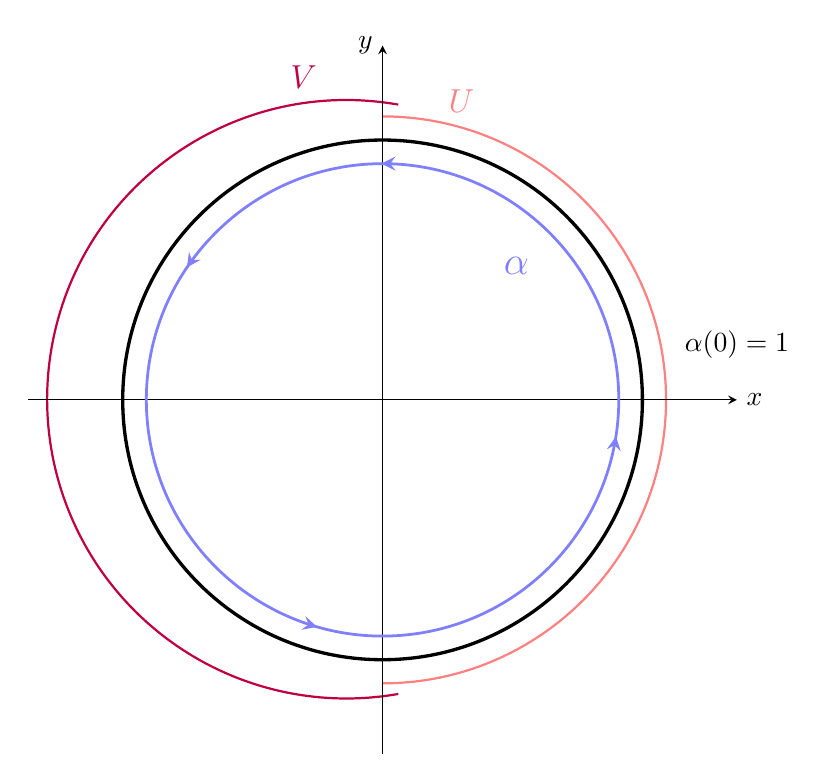
\begin{tikzpicture}[, >= stealth]
                \def\rad{0.8}
                \def\gap{0.2}
                \def\bigradius{3}
                \def\littleradius{0.5}
                
                \draw[red!50, thick] (0, -3.6) arc (-90:90:3.6) node
                at (1, 3.8) {$\mathlarger{\mathlarger{U}}$};

                \draw[purple!100, thick] (0.2, 3.75) arc (-280:-80:3.8) node
                at (-1, 4.1) {$\mathlarger{\mathlarger{V}}$};

                \draw[very thick] (0,0) circle (3.3cm) node at (4.5,
                0.7) {$\alpha(0) = 1$};
                \draw[->] (-4.5,0) -- (4.5,0) node[anchor=west]{$x$};
                \draw[->] (0,-4.5) -- (0,4.5) node[anchor=east]{$y$}; 
                % Red path
                \draw[blue!50, line width=1pt,   decoration={ markings,
                mark=at position 0.2455 with {\arrow[line width=1.2pt]{>}},
                mark=at position 0.4 with {\arrow[line width=1.2pt]{>}},
                mark=at position 0.7 with {\arrow[line width=1.2pt]{>}},
                mark=at position 0.97 with {\arrow[line width=1.2pt]{>}}},
                postaction={decorate}] node at (1.7, 1.7) {$\mathlarger{\mathlarger{\mathlarger{\alpha}}}$}
                let
                \n1 = {asin(\gap/2/\bigradius)},
                \n2 = {asin(\gap/2/\littleradius)}
                in (\n1:\bigradius) arc (\n1:360-\n1:\bigradius)
                -- cycle; 
            \end{tikzpicture}
        \end{figure}

        Since $U$ is not all of $\mathbb{S}^1$, we know that
        $\omega^{-1}(U)$ exists. If we define $\omega(0) = 1$
        (i.e., if we specify that our rotation starts at $1$)
        then $\omega^{-1}(U)$ will correspond to a union of open
        sets around every integer in $\mathbb{R}$. Also,
        $\omega^{-1}(V)$ will correspond to a union of intervals,
        each of which do not intersect any member of $\mathbb{Z}$.
        \begin{figure}[h!]
        \centering 
            \hspace{1mm}
            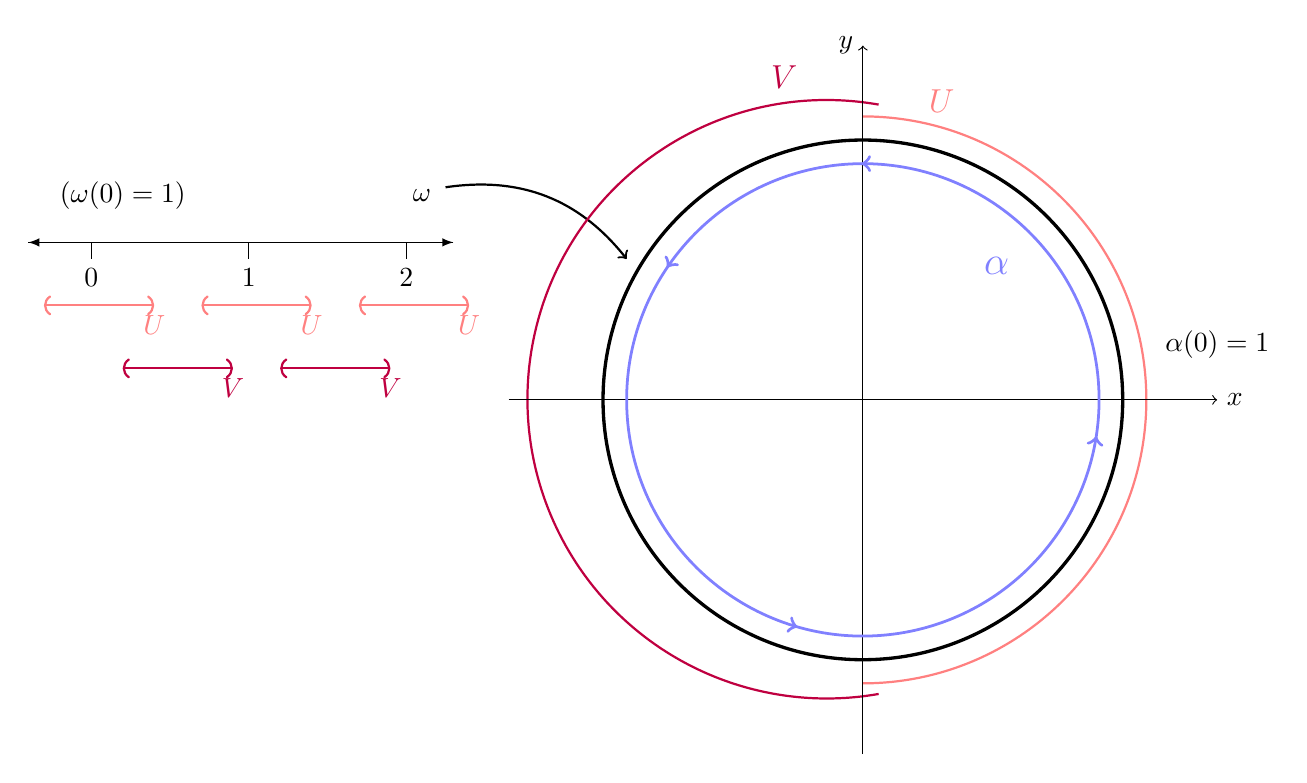
\begin{tikzpicture}
                \def\whatc{red!50}
                \def\whatcc{purple}
                \draw[scale = 2, latex-] (-5.3,1) -- (-2.6,1)
                node at (-2.8, 1.3) {$\omega$};
                \draw[scale = 2, -latex] (-5.3,1) -- (-2.6,1) node at
                (-4.7, 1.3) {($\omega(0) = 1$)};
                \foreach \x in {0,1,2}
                \draw[scale = 2, shift={(\x-4.9,1)},color=black] (0 pt,0pt) -- (0 pt,-3pt) node[below] 
                {$\x$};
                \path[thick, ->] (-5.3, 2.7) edge [bend left] (-3,
                1.79);
                \draw[thick, \whatc, scale = 2, (-)] (-5.2,0.6) --
                (-4.5,0.6)
                node[below, below] {$U$};
                \draw[thick, \whatcc, scale = 2, (-)] (-4.7,0.2) --
                (-4.0,0.2) node[below] {$V$};
                \draw[thick, \whatc, scale = 2, (-)] (-4.2,0.6) --
                (-3.5,0.6) node[below] {$U$};
                \draw[thick, \whatcc, scale = 2, (-)] (-3.7,0.2) --
                (-3,0.2) node[below] {$V$};
                \draw[thick, \whatc, scale = 2, (-)] (-3.2,0.6) --
                (-2.5,0.6)
                node[below] {$U$};

                \def\rad{0.8}
                \def\gap{0.2}
                \def\bigradius{3}
                \def\littleradius{0.5}
                
                \draw[\whatc, thick] (0, -3.6) arc (-90:90:3.6) node
                at (1, 3.8) {$\mathlarger{\mathlarger{U}}$};

                \draw[\whatcc, thick] (0.2, 3.75) arc (-280:-80:3.8) node
                at (-1, 4.1) {$\mathlarger{\mathlarger{V}}$};

                \draw[very thick] (0,0) circle (3.3cm) node at (4.5,
                0.7) {$\alpha(0) = 1$};
                \draw[->] (-4.5,0) -- (4.5,0) node[anchor=west]{$x$};
                \draw[->] (0,-4.5) -- (0,4.5) node[anchor=east]{$y$}; 
                % Red path
                \draw[blue!50, line width=1pt,   decoration={ markings,
                mark=at position 0.2455 with {\arrow[line width=1.2pt]{>}},
                mark=at position 0.4 with {\arrow[line width=1.2pt]{>}},
                mark=at position 0.7 with {\arrow[line width=1.2pt]{>}},
                mark=at position 0.97 with {\arrow[line width=1.2pt]{>}}},
                postaction={decorate}] node at (1.7, 1.7) {$\mathlarger{\mathlarger{\mathlarger{\alpha}}}$}
                let
                \n1 = {asin(\gap/2/\bigradius)},
                \n2 = {asin(\gap/2/\littleradius)}
                in (\n1:\bigradius) arc (\n1:360-\n1:\bigradius)
                -- cycle; 
            \end{tikzpicture}
        \end{figure}

    Now since $\alpha\left(\left[ \frac{i -1 }{N}, \frac{i}{N}
    \right]\right) \subset U$ or $V$, we can map this image to
    $\mathbb{R}$ via $\omega^{-1}$, starting from the first
    interval $\left[ 0, \frac{1}{N} \right]$ which is mapped to a
    neighborhood of $0$ in $\mathbb{R}$. Thus we can define a
    function $\tilde{\alpha}$ as 
    \[
        \tilde{\alpha} = \omega^{-1} \circ \alpha
    \]
    if we specify that $w(0) = 1$ and $\tilde{\alpha}: [0, 1] \to
    \mathbb{R}$ by construction. Therefore, we can write 
    \[
        \alpha = \omega \circ \tilde{\alpha}  
    \]
    where $\alpha(0) = 0$.
    
    \item[2.] Since $\alpha(1) = \alpha(0)$, we see that
    $\alpha$ must return to $U$ at some point. And since there we
    can subdivide $[0, 1]$ into finite intervals to keep track of
    the mapping, there will always be at most a finite number of
    rotations made around $\mathbb{S}$.
    \\
    \\
    Now let us shrink $U$ containing $1$ in $\mathbb{S}$. 
    As we shrink around 1, $\omega^{-1}(U)$ will still be a union of 
    nieghborhoods of integers in $\mathbb{R}$. And since we are to free
    to shrink $U$, we see that the value of $\tilde{alpha}$ 
    must be an integer. 
    \\
    \\
    If $\tilde{\alpha}(1)$ is not an integer, 
    then we can shrink $U$ in $\mathbb{R}$ past this non-integer
    value. However, this implies that $\alpha$ is not a closed
    curve in $\mathbb{S}^1$ since 
    $\alpha(1) \ne \alpha(0)$. Hence, $\omega^{-1}\circ \alpha =
    \tilde{\alpha}$ takes on integer values. 
    \begin{figure}[h!]
        \centering 
            \hspace{1mm}
            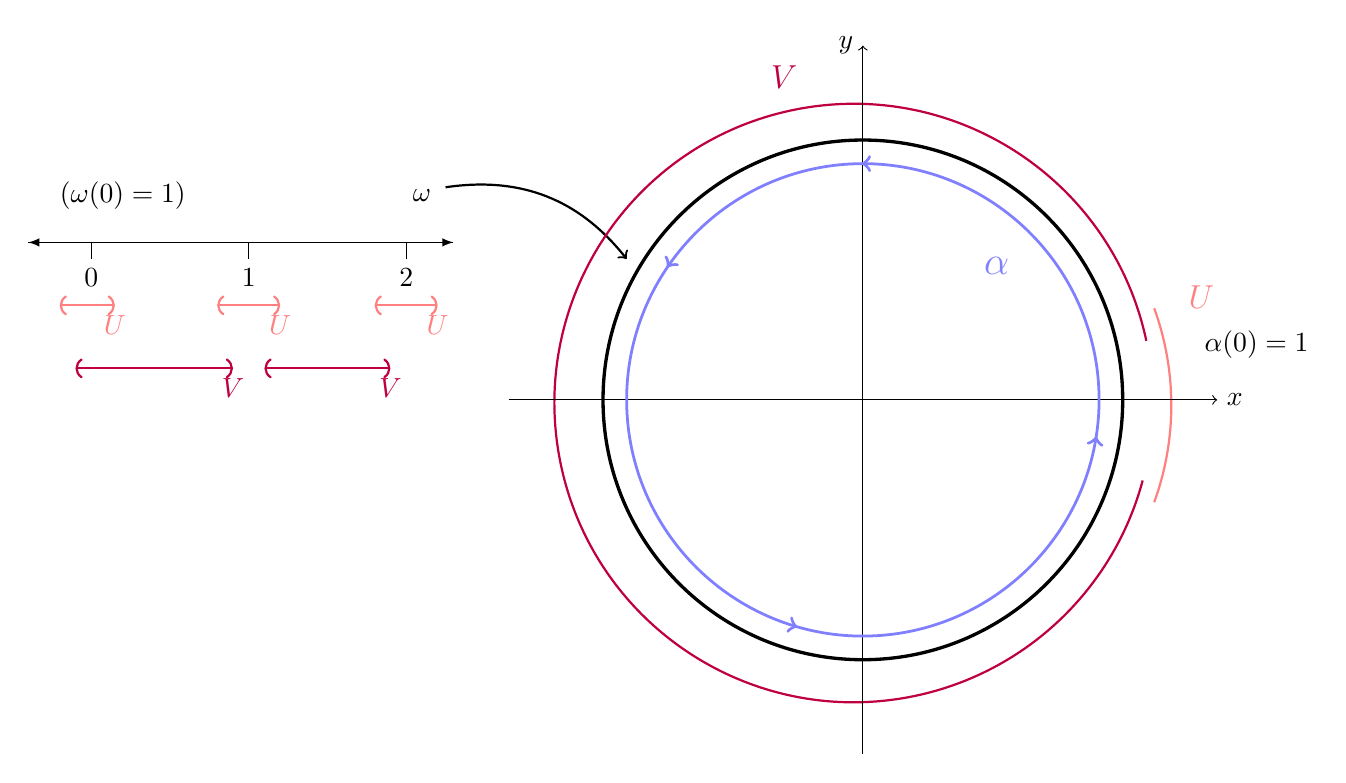
\begin{tikzpicture} 
                \def\whatc{red!50}
                \def\whatcc{purple}
                \draw[scale = 2, latex-] (-5.3,1) -- (-2.6,1)
                node at (-2.8, 1.3) {$\omega$};
                \draw[scale = 2, -latex] (-5.3,1) -- (-2.6,1) node at
                (-4.7, 1.3) {($\omega(0) = 1$)};
                \foreach \x in {0,1,2}
                \draw[scale = 2, shift={(\x-4.9,1)},color=black] (0 pt,0pt) -- (0 pt,-3pt) node[below] 
                {$\x$};
                \path[thick, ->] (-5.3, 2.7) edge [bend left] (-3,
                1.79);
                \draw[thick, \whatc, scale = 2, (-)] (-5.1,0.6) --
                (-4.75,0.6)
                node[below, below] {$U$};
                \draw[thick, \whatcc, scale = 2, (-)] (-5,0.2) --
                (-4.0,0.2) node[below] {$V$};
                \draw[thick, \whatc, scale = 2, (-)] (-4.1,0.6) --
                (-3.7,0.6) node[below] {$U$};
                \draw[thick, \whatcc, scale = 2, (-)] (-3.8,0.2) --
                (-3,0.2) node[below] {$V$};
                \draw[thick, \whatc, scale = 2, (-)] (-3.1,0.6) --
                (-2.7,0.6)
                node[below] {$U$};

                \def\rad{0.8}
                \def\gap{0.2}
                \def\bigradius{3}
                \def\littleradius{0.5}
                
                \draw[\whatc, thick] (3.7, -1.3) arc (-20:20:3.6) node
                at (4.3, 1.3) {$\mathlarger{\mathlarger{U}}$};

                \draw[\whatcc, thick] (3.6,0.75) arc (-348:-15:3.8) node
                at (-1, 4.1) {$\mathlarger{\mathlarger{V}}$};

                \draw[very thick] (0,0) circle (3.3cm) node at (5,
                0.7) {$\alpha(0) = 1$};
                \draw[->] (-4.5,0) -- (4.5,0) node[anchor=west]{$x$};
                \draw[->] (0,-4.5) -- (0,4.5) node[anchor=east]{$y$}; 
                % Red path
                \draw[blue!50, line width=1pt,   decoration={ markings,
                mark=at position 0.2455 with {\arrow[line width=1.2pt]{>}},
                mark=at position 0.4 with {\arrow[line width=1.2pt]{>}},
                mark=at position 0.7 with {\arrow[line width=1.2pt]{>}},
                mark=at position 0.97 with {\arrow[line width=1.2pt]{>}}},
                postaction={decorate}] node at (1.7, 1.7) {$\mathlarger{\mathlarger{\mathlarger{\alpha}}}$}
                let
                \n1 = {asin(\gap/2/\bigradius)},
                \n2 = {asin(\gap/2/\littleradius)}
                in (\n1:\bigradius) arc (\n1:360-\n1:\bigradius)
                -- cycle; 
            \end{tikzpicture}
        \end{figure}
        \item[3.] Suppose $\tilde{\alpha}_1(1) =
        \tilde{\alpha}_2(1)$. Note that $\tilde{\alpha_1}(0) =
        \tilde{\alpha_2(0)}$, and as these are paths in
        $\mathbb{R}$ we can construct a stright line homotopy
        between the two paths relative to $\{0, 1\}$. Thus
        $\tilde{\alpha_1} \sim \tilde{\alpha_2}$, and there exists
        a homotopy $H$ from $\tilde{\alpha_1}$ to $\tilde{\alpha_2}$. 
        \\
        \\
        Since $\omega$ is continuous, 
        $\omega \circ H$ is a continuous and a homotopy between $\alpha_1$ and
        $\alpha_2$, since (1) $(\omega \circ H)(0, t) = \omega
        \circ \tilde{\alpha_1} = \alpha_1$ and (2) $(\omega \circ
        H)(1, t) = \omega \circ \tilde{\alpha_2} = \alpha_2$,
        and the homotopy retains the endpoints. 

        \item[4.] Now consider the function $\gamma: \mathbb{S} \to
        \mathbb{Z}$ given by 
        \[
            \phi(\gamma) = \tilde{\gamma}(1).
        \]
        Let $\gamma_1, \gamma_2 \in \pi_1(\mathbb{S}^1)$. Then
        observe that $\gamma_1 \cdot \gamma_2$ will be a path
        which comples $\tilde{\gamma}_1$ rotations, followed by
        $\tilde{\gamma}(2)$ rotations. Therefore 
        \[
           \phi(\gamma_1 \cdot \gamma_2)
           = \tilde{\gamma_1}(1) + \tilde{\gamma_2}(1) = \phi(\gamma_1) + \phi(\gamma_2).
        \]
        Thus $\phi$ is a homomorphism. Now observe that part (3)
        of this problem proves injectivity, while surjectivity
        comes from the fact that for any $n \in \mathbb{Z}$, we
        can create a loop $\alpha$ such that $\alpha$ completes
        $n$ rotations in $\mathbb{S}$, giving that
        $\tilde{\alpha}(1) = n$. Therefore $\phi$ is bijective and
        hence an isomorphism, so that $\pi_1(\mathbb{S}) \cong \pi_1(\mathbb{Z})$.
        
    \end{itemize}

\end{proof}

\begin{problem}[Theorem 13.15]
    Let $(X, x_0), (Y, y_0)$ be path connected spaces. Then 
    \[
        \pi_1(X \times Y, (x_0, y_0)) \cong \pi_1(X, x_0) \times \pi_1(Y, y_0)
    \]
    via the canonical map that takes a loop $\gamma$ in $X \times Y$
    to $(p \circ \gamma, q \circ \gamma)$ where $p: X \times Y \to X$
    and $q : X \times Y \to Y$ are projection maps. 
\end{problem}

\begin{proof}
    Observe that the map $(p \circ \gamma, q \circ \gamma)$ as defined
    above is a homomorphism. To show this, let $\gamma \in \pi_(X
    \times Y, (x_0, y_0))$. Then 
    \[
        \phi(\gamma) = (p \circ \gamma, q \circ \gamma) = (\gamma_x, \gamma_y) =
        (\gamma_x, e_{y_0}) \cdot (e_{x_0}, \gamma_y) = \phi(\gamma_x)\cdot\phi(\gamma_y)
    \]
    where $\gamma_x$ is a loop in $X$ based at $x_0$, $\gamma_y$ a
    loop in $Y$ based at $y_0$. Observe that this is bijective since
    every loop in $\pi_1(X \times Y, (x_0, y_0))$ is mapped to a loop
    in $\pi_1(X, x_0) \times \pi_1(Y, y_0)$, and every loop in
    $\pi_1(X, x_0) \times \pi_1(Y, y_0)$ can be written as a loop in 
    $\pi_1(X \times Y, (x_0, y_0))$. Therefore this is a isomorphism
    and thus $\pi_1(X \times Y, (x_0, y_0)) \cong \pi_1(X, x_0) \times \pi_1(Y, y_0)$
\end{proof}



\begin{exercise}[Exercise 13.16]Find:
\begin{itemize}
    \item[1.] $\pi_1(X)$ where $X$ is a solid torus.
    \item[2.] $\pi_1(\mathbb{S}^2 \times \mathbb{S})$
    \item[3.] $\pi_1(\mathbb{S}^2\times \mathbb{S}^2 \times \mathbb{S}^2)$
    \item[4.] $\pi_1(X)$, where $X$ is a direct product of $k_n$
    copies of $\mathbb{S}^n$, with $k_n = 0$ for $n$ sufficiently
    large.
\end{itemize}
\end{exercise}


\begin{exercise}[Exercise 13.18] 
Check that for a continuous function $f : X
\to Y$, the induced homomorphism $f_*$ is well-defined (that is, the
image of an equivalence class is independent of the chosen
representative.) Show that it is indeed a group homomorphism.
\end{exercise}

\begin{solution}
Observe that since $\alpha \sim \beta$, there exists a homotopy
$H$ between the two paths that fixes the endpoints. Then observe
that $f \circ H$ is (1) a continuous function and (2) a homotopy 
from $f(\alpha)$ to $f(\beta)$. Thus $f(\alpha) \sim f(\beta)$.
Therefore, 
if $\alpha \sim \beta$ then $f(\alpha) \sim f(\beta) 
\implies [f \circ \alpha] = [f \circ \beta] \implies 
f_*([\alpha]) = f_*([\beta])$ so that our definition is
well defined.
\\
\\
To show it is a group homomorphism, observe that 
\[
  f_*([\alpha \cdot \beta]) = [f \circ (\alpha \cdot \beta)]
  = [f \circ \alpha \cdot f \circ \beta] = [f \circ \alpha] \cdot [f \circ \beta]
  = f_*([\alpha]) \cdot f_*([\beta]).
\]
Thus we see that this forms a group homomorphism. 
\end{solution}


\begin{problem}[Theorem 13.19]
    The following are true:
    \begin{itemize}
        \item[1.] If $f: (X, x_0) \to (Y, y_0)$ and $g: (Y, y_0)
        \to (Z, z_0)$ are continuous maps, then $(g \circ f)_* = g_*
        f_*.$
        
        \item[2.] If $\text{id}:(X, x_0) \to (Y, y_0)$ is the identity
        map, then $\text{id}_*: \pi_1(X, x_0) \to \pi_1(X, x_0)$ is
        the identity homomorphism.        
    \end{itemize}
\end{problem}

\begin{proof}
    \begin{itemize}
        \item[1.] Let $[\alpha] \in \pi_1(X, x_0)$. 
        Then 
        \[
            (g \circ f)_*([\alpha]) = [(g \circ f) \circ \alpha] 
            = [g \circ (f \circ \alpha)]
            = g_*([f_*([\alpha])]) = g_* \circ f_*([\alpha]) 
        \]
        so that $(g \circ f)_* = g_*f_*$.
        
        \item[2.] Let $[\alpha] \in \pi_1(X, x_0)$. Then 
        \[
            id_*([\alpha]) = [id \circ \alpha] = [\alpha].
        \]
        Since this is a homomorphism on the group which sends every
        group element to itself, we have that this is an identity homomorphism.
    \end{itemize}
\end{proof}

\begin{problem}[Theorem 13.20]
    If $h: X \to Y$ is a homeomorphism then 
    \[
        h_*: \pi_1(X, x_0) \to \pi_1(Y, y_0)       
    \]
    is a group isomorphism. Thus homeomorphic, path-connected spaces
    have isomorphic fundamental groups.
\end{problem}

\begin{proof}
    If $h: X \to Y$ is a homeomorphism, then $h$ is continuous and
    bijective. Therefore, if $\alpha \in \pi_1(X, x_0)$, then 
    $h_* = [h \circ \alpha]$. Since $h^{-1}$ exists and is continuous,
    we then now if $\beta \in \pi_1(Y, y_0)$ then 
    $h^{-1}_* = [h^{-1} \circ \alpha]$ is also a homomorphism. Now
    observe that 
    \begin{gather*}
        h_*[h^{-1}_*[\beta]] = [h \circ [h^{-1} \circ \beta]] = [\beta]\\
        h^{-1}_*[h_*[\alpha]] = [h^{-1} \circ [h \circ \alpha]] = [\alpha].
    \end{gather*}
    Therefore, we see that $h^{-1}_*$ is the inverse homomorphism of
    $h_*$, which implies that the homomorphism is bijective.
    Therefore, the two groups are isomorphic.
\end{proof}



\begin{problem}[Theorem 13.22]
    If $f, g : (X, x_0) \to (Y, y_0)$ are continuous functions and $f$
    is homotopic to $g$ relative to $x_0$, then $f_* = g_*$.
\end{problem}

\begin{proof}
    Since $f \simeq g$, there exists a homotopy $H$ such that $H(x, 0)
    = f(x), H(x, 1) = g(x)$ and $H(x_0, t) = f(x_0) = g(x_0)$ for all
    $t \in [0, 1]$. Let $\alpha \in \pi_1(X, x_0)$. Then observe that 
    $H(\alpha(x), t)$ is (1) continuous and (2) a homotopy from $f
    \circ \alpha$ to $g \circ \alpha$. Therefore 
    \[
        f \circ \alpha \simeq g \circ \alpha \implies [f \circ \alpha] = [g \circ \alpha]
        \implies f_* = g_*.
    \]
\end{proof}

\begin{problem}[Lemma 13.23]
    Homotopy equivalence of spaces is an equivalence relation.
\end{problem}

\begin{proof}
    We can show that this satisfies the axioms for an equivalence
    relation.
    \begin{description}
        \item[Reflexive.] Observe that if we let $f = g = id_X$,
        then $g \circ f = id_X$ and $f \circ g = id_X$. 
        Thus a topological space $X$ is homotopy
        equivalent to itself. 

        \item[Symmetric.] The defintion of homotopy equivalence makes
        this obvious.
        Suppose $X$ is homotopy equivalent to $Y$.
        By definition, there exists continuous maps $f: X \to Y$ and
        $g: Y \to X$ such that 
        \[
            g \circ f \simeq id_X \qquad f \circ g \simeq id_Y.  
        \]
        Thus $Y$ is homotopy equvalent to $X$ since there exists
        continuous functions $g: Y \to X$ and $f: X \to Y$ such that 
        \[
            f \circ g \simeq id_Y \qquad g \circ f \simeq id_X.  
        \]

        \item[Transitive.] Suppose $X$ is homotopy equivalent to $Y$
        which is homotopy equivalent to $Z$. By definition, there
        exist continuous functions $f_1 : X \to Y$, $f_2: Y \to X$, 
        $g_1 : Y \to Z$, $g_2 : Z \to Y$ such that 
        \[
            f_1 \circ f_2 \simeq id_X \qquad f_2 \circ f_1 \simeq id_Y
            \text{ and } g_1 \circ g_2 \simeq id_Y \qquad g_2 \circ g_1 \simeq id_Z
        \]
        
    \end{description}
\end{proof}

\begin{problem}[Theorem 13.24]
    If $f: X \to Y$ is a homotopy equivalence and $y_0 = f(x_0)$, then
    $f_* : \pi_1(X, x_0) \to \pi_1(Y, y_0)$ is an isomorphism. In
    particular, if $X \sim Y$, then $\pi_1(X) \cong \pi_1(Y)$.
\end{problem}

\begin{proof}
    Since $f$ is continuous from $X$ to $Y$, we already have a
    homomorphism from $\pi_1(X, x_0) \to \pi_1(Y, y_0)$, given by
    $f_*.$ Now consider the induced homomorphism $g_*$ where 
    \[
        g \circ f \simeq id_X \quad \text{and} \quad f \circ g \simeq id_Y.
    \]
    Then observe that if $\alpha \in \pi_1(X, x_0)$ then
    \[
        g_* \circ f_*[\alpha] = (g_* \circ f_*)[\alpha] = [g \circ f \circ \alpha].
    \]
    Now since $g \circ f \simeq id_X$, we know that there exists a
    homotopy $H$ such that $H(x, 0) = g \circ f$ and $H(x, 1) = id_X$
    while $H(x_0, t) = g \circ f(x_0) = id_X(x_0) = x_0.$ Then observe
    that $H(\alpha(x), t)$ is a homotopy from $g \circ f \circ \alpha$
    to $\alpha$. As these two paths are homotopic, their equivalence
    classes should be the same. Therefore, we see that 
    \[
        [g \circ f \circ \alpha] = [\alpha].
    \]
    Now if $\beta \in \pi_1(Y, y_0)$
    \[
        f_* \circ g_*[\beta] = (f_* \circ g_*)[\beta] = [f \circ g \circ \beta]= [\beta]
    \]
    By the same argument. Therefore, $g_*$ is an inverse homomorphism of $f_*$, so that
    $f_*$ is ultimately an isomorphism between the two groups.
    Thus $\pi_1(X, x_0) \cong \pi_1(Y, y_0)$.
\end{proof}

\begin{exercise}[Exercise 13.25]
Show that for $n \ge 0$, $\mathbb{R}^{n + 1}-\{0\}$ can be strong
deformation retracted onto $\mathbb{S}^n$
\end{exercise}

\begin{solution}
Consider the homotopy $R : \mathbb{R}^{n+1} \to \mathbb{S}^n$ such
that 
\begin{gather*}
    R(\mathbf{x}, 0) = \mathbf{x} \quad \text{ for all } \mathbf{x} \in \mathbb{R}^{n+1} \\
    R(x, 1) = r(x) \quad \text{ for all } \mathbf{x} \in \mathbb{R}\\
    R(a, t) = a \quad \text{ for all } a \in \mathbb{S}^n
\end{gather*}
where 
\[
   r(\mathbf{x}) = \frac{\mathbf{x}}{||\mathbf{x}||}. 
\]
Thus we see that 
$\mathbb{R}^{n + 1}-\{0\}$ can be strong
deformation retracted onto $\mathbb{S}^n$.
\end{solution}

\begin{problem}[Lemma 13.26]
    If $A$ is strong deformation retract of $X$, then $A$ and $X$ are
    homotopy equivalent.
\end{problem}

\begin{proof}
    Since $A$ is a strong deformation retract of $X$, we know that
    there exists a continuous function $r: X \to A$ such that $r(a) =
    a$ for all $a \in A$. Consider also the inclusion map $i: A \to
    X$. Observe that 
    \[
        i \circ r : X \to X \quad  r \circ i: A \to A
    \]
    and 
    \[
        r \circ i = id_A \quad  i \circ r \simeq id_X.
    \]
    Thus by defintion we see tha $A \sim X$.
\end{proof}

\begin{problem}[Theorem 13.27]
    $\mathbb{R}^2$ is not homeomorphic to $\mathbb{R}^n$, for any $n
    \ne 2$.
\end{problem}

\begin{proof}
    Suppose for contradiction that $\mathbb{R}^2$ is homeomorphic to 
    $\mathbb{R}^n$. Then if we poke a hole in $\mathbb{R}^2$, we can
    embed a circle in the space such that its interior contains the
    hole. We can then strong deformation retract $\mathbb{R}^2$ onto
    the boundary of the disk. We then see the fundamental
    group is $\mathbb{Z}$ by Theorem 13.24. 
    \\
    \\
    However, we know that $\mathbb{R}^n$, $n \ge 2$ with one hole
    missing is still a trivial group. In $\mathbb{R}^n$, we can move
    around the circle we embdedded in $\mathbb{R}^2$ to still compute
    a trivial fundamental group. But this is a contradiction, since
    these two spaces are said to be homeomorphic but their fundamental
    groups are inconsistent under change. Therefore, $\mathbb{R}^2$ is
    not homeomorphic to $\mathbb{R}^n$ for any $n \ge 2$.
    \\
    \\
    Also observe that $\mathbb{R}^2$ is not homemorphic to
    $\mathbb{R}$. This is because $\pi_1(\mathbb{R}^2) \cong
    \mathbb{R} \times \mathbb{R}$. Also, $\mathbb{R}^2$ is not
    homeomorphic to $\mathbb{R}^{0}$, as this is a single point. If we
    delete this point the fundamental group is empty, while the
    fundamental group of $\mathbb{R}^2$ would become equivalent to
    $\mathbb{Z}$, and hence these two spaces are not homemorphic. 
    Therefore, we see that $\mathbb{R}$ is not homeomorphic to
    $\mathbb{R}^n$ for any $n \ne 2$.

\end{proof}

\begin{exercise}[Exercise 13.28]
Let $x$ and $y$ be two points in $\mathbb{R}^2$. Show that
$\mathbb{R}^2 - \{x, y\}$ strong deformation retracts onto the figure
eight. In addition, show that $\mathbb{R}^2$. Show that
$\mathbb{R}^2 - \{x, y\}$ strong deformation retracts onto a theta
space.
\end{exercise}

\begin{solution}
Observe that the figure eight and the theta space both have two holes
inside of them. If we configure both of these holds to individually
contain $x$ and $y$, then we can retract $\mathbb{R}$ ont the
boundaries of the figure eight and theta space. 
\\
\\
Note we would not be able to do this without first poking two holes in
$\mathbb{R}$, since we would otherwise not be able to retract the
interior of the each hole in the figure eight or theta space to its
boundaries (for the same reason we can't retract $\mathbb{D}^2$ to its
boundary).
\end{solution}
    
\begin{problem}[Theorem 13.29]
    If $r : X \to A$ is a strong deformation retraction and $a \in A$,
    then $\pi_1(X, a) \cong \pi_1(A, a)$.
\end{problem}

\begin{proof}
    Suppose $r: X \to A$ is a strong deformation retraction. Then by
    Lemma 13.26, we know that $A$ and $X$ are homotopy equivalent.
    Moreover, by Theorem 13.24, we have that $\pi_1(X,a) \cong
    \pi_1(A, a)$ for $a \in A$. 
\end{proof}

\begin{exercise}[Exercise 13.30]
    Calculate the fundamental group of the following spaces.
    \begin{itemize}
        \item[1.] An annulus.
        \item[2.] A cylinder.
        \item[3.] The Möbius Band.
        \item[4.] An open 3-ball with a diameter removed.   
    \end{itemize}
\end{exercise}

\begin{solution}
    \begin{itemize}
        \item[1.] Suppose that we embed an annulus at the origin of the complex
        plane. Then it is given by $\{z : R_1 < |z| < R_2\}$ where
        $R_1 < R_2$. It should be fairly obvious that we can construct
        a strong deformation retract
        to the set of points $\{z : |z| = R_1\}$; that is, to the
        inner circle of the annulus. As the fundamental group of the
        circle is $\mathbb{Z}$, we can thus conclude that the
        fundamental group of the annulus is also $\mathbb{Z}$ by
        Theorem 13.29.

        \item[2.] For a cylinder, we can embedd such a structure in
        $\mathbb{R}^3$, which in this space we can construct a
        strong deformation retract between the set of points on the
        cylinder to one of the two disks which define the top and
        the bottom of the cylinder. Since the fundamental group of a
        disk is trivial, we see that the fundamental group of the
        cylinder must also be trivial by Theorem 13.29.

        \item[3.] Observe that if we take a Möbius band and strong
        deformation retract the set of points to one of its
        boundaries, we'll get a closed curve, which we can then form a
        strong deformation retraction to a circle. Since the
        fundamental group of a circle is $\mathbb{Z}$, we see that the
        fundamental group of the Möbius band is also $\mathbb{Z}$. 
        \\
        \\
        However, if the cylinder does not have a filled top (i.e., the
        cylinder is just a piece of paper folded on its ends) then the
        group is trivial 

        \item[4.] Observe that we can strong deformation retract an
        open 3-ball with a diameter removed to a circle with a hole
        removed from its center. Since this has a fundamental group of
        $\mathbb{Z}$, we see that by Theorem 13.27 that the open
        3-ball with diameter removed also has a fundamental group of 
        $\mathbb{Z}$.

    \end{itemize}

\end{solution}



\begin{problem}[Theorem 13.32]
    Let $A$ be a retract of $X$ via the inclusion $i : A
    \xhookrightarrow{} X$ and retraction $r: X \xhookrightarrow{} A$.
    Then for $a \in A$, $i_* : \pi_1(A, a) \to \pi_1(X, a)$ is
    injective and $r_*: \pi_1(X, a) \to \pi_1(A, a)$ is surjective. 
\end{problem}

\begin{proof}
    First note that for any
    $\alpha \in \pi_1(A, a)$ we have that 
    \[
        r_* \circ i_*([\alpha]) = [r \circ i \circ \alpha] = [\alpha].
    \]
    Therefore, we see that $ r_* \circ i_*([\alpha]) = id_*$ 
    is the identity homomorphism on $\pi_1(A, a)$. 
    Now suppose that $i_*$ is not injective. Then we'll have that 
    $r_* \circ i_* \ne id_*$, which is a contradiction. Furthermore,
    if $r_*$ is not surjective then $r_* \circ i_* \ne id_*$. Thus we
    see that $i_*$ is injective and $r_*$ is surjective.
\end{proof}

\begin{problem}[Theorem 13.33] 
    (No retraction theorem for $\mathbb{D}^2$.) There is no retraction
    from $\mathbb{D}^2$ to its boundary.
\end{problem}

\begin{proof}
    Suppose for a contradiction that there exists a retraction $r :
    \mathbb{D}^2 \to \mathbb{S}^1$. Then the inclusion map $i_* :
    \pi_1(\mathbb{S}^1) \to \pi_1(\mathbb{D}^2)$ should be injective,
    this is impossible since $\pi_1(\mathbb{S}^1) = \mathbb{Z}$ while
    $\pi_1(\mathbb{D}^2)$ is trivial. Thus there is no such $r$.
\end{proof}

\newpage
\begin{problem}[Theorem 13.34]
    (Brouwer Fixed Point Theorem for $\mathbb{D}^2$.) Let $f:
    \mathbb{D}^2 \to \mathbb{D}^2$ be a continuous map. Then there is
    some $x \in \mathbb{D}^2$ for which $f(x) = x.$
\end{problem}

\begin{proof}
    Suppose for a contradiction that there exists a continuous
    function $f: \mathbb{D}^2 \to \mathbb{D}^2$ such that $f(x) \ne x$
    for all $x \in \mathbb{D}^2$. Consider the retraction $\phi(x) =
    x$ if $x \in \mathbb{S}^1$ and $\phi(x) = f(x)|_\text{proj}$ where
    $f(x)_\text{proj}$ is the projection of $f(x)$ to its boundary
    through the straightline between $f(x)$ and $x$.
    \begin{figure}[h!]
        \centering        
        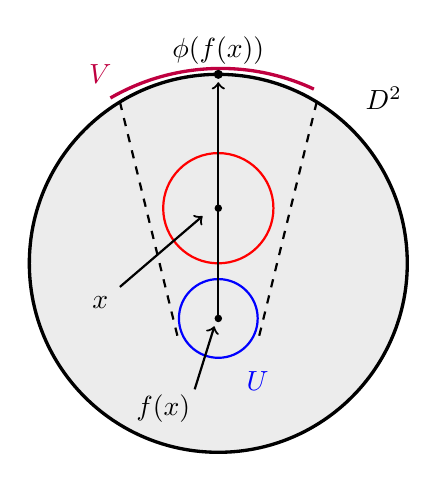
\begin{tikzpicture}
            %circles
            \draw[very thick, purple] (-1.37, 2.1) arc (120:65:2.8)
            node at (-1.5, 2.4) {$V$};
            \filldraw[gray!15, very thick] (0,0) circle (2.4cm) node at (2.1, 2.1)
            {$\color{black}\mathbb{D}^2$};
            \draw[blue, thick] (0,-0.7) circle (0.5cm)node at (0.5, -1.5) {$U$};
            \draw[red, thick] (0,0.7) circle (0.7cm);
            \draw[very thick, black] (2.4,0) arc(0:360:2.4);

            %lines
            \draw[dashed, black, thick] (-1.25,2.05) -- (-0.5,-1);
            \draw[dashed, black, thick] (1.25, 2.05) -- (0.5,-1);
            \draw[thick, ->] (0, -0.7) -- (0, 2.3);

            %labeling
            \draw[thick, ->] (-0.3, -1.6) -- (-0.05, -0.8) node at
            (-.7, -1.85) {$f(x)$};
            \draw[thick, ->] (-1.25, -.3) -- (-0.2, 0.6) node at
            (-1.5, -.5) {$x$};
            \filldraw (0,0.7) circle (0.4mm); %f(x)
            \filldraw (0,-0.7) circle (0.4mm); %x$
            \filldraw (0, 2.4) circle (0.5mm) node[above] {$\phi(f(x))$}; %\phi(f(x))
        \end{tikzpicture}
    \end{figure}

    Observe that this function is continuous, since for any open set
    containing $V \subset \mathbb{S}^1$ containing $\phi(f(x))$ there
    exists an open set $U \in 
    \mathbb{D}^2$ containing $f(x)$ such that $\phi(U) \subset V$. See
    the figure. 
    \\

    Note that what we have is a continuous retraction of
    $\mathbb{D}^2$ to its boundary, $\mathbb{R}$. However, we know
    from Theorem 13.33 that this is a contradiction. Thus there cannot
    be any such $f$, so that for a continuous
    $f: \mathbb{D}^2 \to \mathbb{D}^2$ there must exist an $x \in
    \mathbb{D}^2$ such that $f(x) = x$, as desired.


\end{proof}

\begin{problem}[Theorem 13.40]
    Let \(X = U \cup V\), where \(U\) and \(V\) are open and path
    connected and \(U \cap V\) is path-connected, simply connected and
    nonempty. Then \(\pi_1(X) \cong \pi_1(U) \star \pi_1(V).\)
\end{problem}

\begin{proof}
    Let $x_0 \in U \cap V$ and let $\Gamma$ be a loop based at $x_0$.
    Then observe that $\Gamma: [0, 1] \to X$ is a path from a compact
    interval, and $U$ and $V$ form an open cover of $X$.
    By Theorem 10.25 we may divide the interval into
    finite subintervals such that the image of each interval lies in
    $U$ or $V$. 
    \\
    \\
    We now claim that we can write any loop $\Gamma$ as product of
    loops in $\pi_1(U)$ and $\pi_1(V)$. Since $U \cap V$ is path
    connected, we know that for every every time our path intersects
    $U \cap V$ there exists a point $p \in U \cap V$ such that we can
    glue a new path $\gamma$ from $p$ to $x_0$. This path will either
    lie entirely in $U$ or in $V$, thus becoming a member of
    $\pi_1(U)$ and $\pi_1(V)$. And by Theorem 10.25, this can be done
    a finite number of times. 
    \\
    \\
    Now consider the function 
    \[
        \phi(\Gamma) = \alpha_1\beta_1 \cdots \alpha_n\beta_n
    \]
    where $\alpha_1\beta_1 \cdots \alpha_n\beta_n$ is the
    decomposition of $\Gamma$ and $\alpha_i \in \pi_1(U)$ while
    $\beta_i \in \pi_i(V)$ for $i = 1, 2, \dots, n.$ We'll now show
    this is a homomorphism. For any two paths $\Gamma_1, \Gamma_2$,
    each have some decomposition $\alpha_1^{(1)}\beta_1^{(1)} \cdots
    \alpha_n^{(1)}\beta_n^{(1)}$ and $\Gamma_2 = \alpha_1^{(2)}\beta_1^{(2)} \cdots
    \alpha_n^{(2)}\beta_n^{(2)}$. Therefore, we see that 
    \[
        \Gamma_1 \cdot \Gamma_2 = \alpha_1^{(1)}\beta_1^{(1)} \cdots
        \alpha_n^{(1)}\beta_n^{(1)}\alpha_1^{(2)}\beta_1^{(2)} \cdots
        \alpha_n^{(2)}\beta_n^{(2)}
    \]
    so that 
    \[
        \phi(\Gamma_1 \cdot \Gamma_2) = \alpha_1^{(1)}\beta_1^{(1)} \cdots
        \alpha_n^{(1)}\beta_n^{(1)}\alpha_1^{(2)}\beta_1^{(2)} \cdots
        \alpha_n^{(2)}\beta_n^{(2)}
        = \phi(\Gamma_1)\phi(\Gamma_2).
    \]
    Thus observe that for any $\alpha_1\beta_1 \cdots
    \alpha_n\beta_n\in \pi_1(X)$, this corresponds to some unique path
    $\Gamma \in pi_1(X)$ such that 
    \[
        \phi(\Gamma) = \alpha_1\beta_1 \cdots
        \alpha_n\beta_n
    \]
    Thus we get surjectivity for free, since any member of
    $\pi_1(U)\star \pi_1(V)$ corresponds to some path $\Gamma \in
    \pi_1(X)$; therefore, the image of $\Gamma$ under $\phi$ is then
    the element of $\pi_1(U)\star \pi_1(V)$ we began with. However,
    this also lends uniqueness, since every member of $\pi_1(U)\star
    \pi_1(V)$ corresponds uniquely to some path of $\Gamma \in
    \pi_1(X)$. Therefore we see that this is a isomorphism, so that
    $\pi_1(X) \cong \pi_1(U)*\pi_1(V)$.
\end{proof}

\begin{exercise}[Exercise 13.41]
     Let $X$ be the bouqeuet of $n$ circles. What
is $\pi_1(X)$?
\end{exercise}

\begin{solution}
The bouquet of $n$ circles simply identifies a point on a set of $n$
circles to the same point. Thus we see by repeated application of
Theorem 13.30, $\pi_1(X) \cong
\pi_1(\mathbb{S})*\pi_1(\mathbb{S})*\dots*\pi_1(\mathbb{S})$ 
= $\mathbb{Z}*\mathbb{Z}*\dots*\mathbb{Z}$. That is, the free product
of $n$ groups of $\mathbb{Z}$.
\end{solution}

\begin{exercise}[Exercise 13.32]
    Find a path-connected space $X$ with open,
path connected subsets $U$ and $V$ of $X$ such that $X = U \cup V$
where $U$ and $V$ are both simply connected, but $X$ is not simply
connected. Conclude that the hypothesis that $U \cap V$ is path
connected is necessary. 
\end{exercise}

\begin{solution}
Consider the sets 
\begin{figure}[h!]
    \centering
    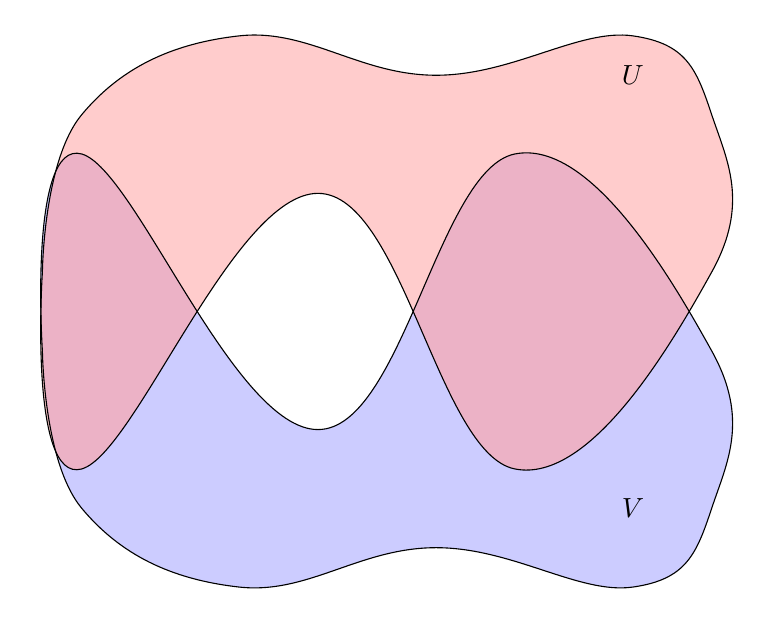
\begin{tikzpicture}
        \def\shapeone{%\draw[fill = red!40, draw = black, thick] 
        plot[smooth, tension=.7] coordinates {(-3.5,0.5)
        (-3,2.5) (-1,3.5) (1.5,3) (4,3.5) (5,2.5) (5,0.5) (2.5,-2)
        (0,1.5) (-3,-2) (-3.5,0.5)};}
        \def\shapetwo{%\draw[fill = blue!40, draw = black, thick] 
        plot[smooth, tension=.7] coordinates {(-3.5,-0.5)
        (-3,-2.5) (-1,-3.5) (1.5,-3) (4,-3.5) (5,-2.5) (5,-0.5)
        (2.5,2) (0,-1.5) (-3,2) (-3.5,-0.5)};}

        \fill[red!20] \shapeone;
        \fill[blue!20] \shapetwo;

        \begin{scope}
            \clip \shapeone;
            \fill[purple!30] \shapetwo;
        \end{scope}

        \draw \shapeone;
        \node at (4, 3) {$U$};
        \draw \shapetwo;
        \node at (4, -2.5) {$V$};
    \end{tikzpicture}
\end{figure}

where we see that $U \cap V$ is not path connected. In this example we
see that the consequence of this is that the union of the sets $U \cup
V$ is no longer simply connected, and hence it has a nontrivial
fundamental group. However, if we were to ignore the condition that
$U \cap V$ be path connected, then Van Kampen's
theorem in this case would otherwise guarantee that its fundamental
group should be the free product of two trivial groups, and hence be a
trivial group itself. Thus path connectedness of $U \cap V$ is a
necessary condition for Van Kampen's theorem to be true.
\end{solution}

\begin{problem}[Theorem 13.44]
    Let $X$ be a wedge of two cones over two Hawaiian earrings where
    they are identified at the points of tangency of the circles of
    each Hawaiian earring, as in Figure 13.9. Then $\pi_1(X) \not\cong
    1$.
\end{problem}

\begin{proof}
    Suppose $\alpha_n$ is a loop on the $n$-th ring on the left
    Hawaiian earring, while $\beta_n$ is a loop on the $n$-th ring on
    the right Hawaiian earing. Thus consider the path 
    \[
        \gamma = \alpha_1\beta_1\alpha_2\beta_2\cdots\alpha_k\beta_k
    \]
    where $k \in \mathbb{N}$. Observe that
    $\gamma \in \pi_1(X)$ (more specifically, its equivalence class is a member).
    However, if we attempt to lift this path towards the
    apex of the cone, which we can individually do without any issue
    for $\alpha_1\alpha_2\cdots\alpha_k$ and
    $\beta_1\beta_2\cdots\beta_k$, we run into an issue as $k \to
    \infty$. This is because $[0, 1]$ is a compact interval and cannot
    be mapped into an infinite path, so that if we attempted to form
    any homotopy it would automatically fail to be compact and hence
    continuous if we try to lift the path $\gamma$ up simultaneously.
    Thus this path is not homotopic to a point, so that $\pi_1(X) \ne
    1$. 




\end{proof}
    



\end{document}